\chapter[\hspace{0pt}基于多粒度样本关系建模的少样本分类研究]{{\heiti\zihao{3}\hspace{0pt}基于多粒度样本关系建模的少样本分类研究}}\label{chapter3: 基于多粒度样本关系建模的少样本分类研究}
\removelofgap
\removelotgap
本章研究基于多粒度样本关系建模的少样本特征学习算法,通过挖掘多种粒度的样本关系并对其进行建模从而增强模型的特征提取能力,进而提升少样本分类任务的准确率。本章内容共分为四节,\hyperref[section3: 引言]{第一节}介绍研究动机和方法概述;\hyperref[section3: 基于多粒度样本关系对比学习的少样本特征学习算法]{第二节}介绍本章提出的基于多粒度样本关系对比学习的少样本特征学习算法;\hyperref[section3: 实验设置及结果分析]{第三节}给出实验设置和结果分析;\hyperref[section3: 本章小结]{第四节}对本章进行小结。

\section[\hspace{-2pt}引言]{{\heiti\zihao{-3} \hspace{-8pt}引言}}\label{section3: 引言}

\subsection[\hspace{-2pt}研究动机]{{\heiti\zihao{4} \hspace{-8pt}研究动机}}\label{section3: 研究动机}

\begin{figure}[h!]
\centering
\captionsetup{font={small, stretch=1.312}}
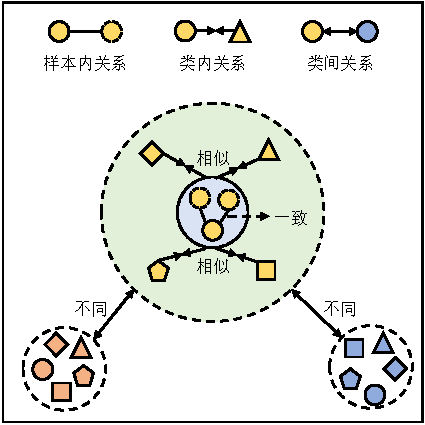
\includegraphics[width=0.6\columnwidth]{figures/MGSRCL/SampleRelation.pdf}
% \captionsetup{justification=justified,singlelinecheck=false}
\bicaption[样本关系示意图]{样本关系示意图。在该图中,不同形状与颜色分别代表不同样本与类别。同一样本的不同变换由相同的颜色和形状表示。样本关系包括三种类型:样本内关系、类内关系和类间关系。本章所提方法约束同一样本不同变换版本在语义内容上保持一致,同类样本保持相似,非同类样本保持不同。}[Illustration of sample relations]{Illustration of sample relations. In this figure, different shapes and different colors represent different samples and different classes, respectively. Different transformations of the same sample are represented by the same color and shape. The sample relations contain three types: intra-sample relation, intra-class relation and inter-class relation. The approach proposed in this chapter enforces different transformations to be consistent in semantic content, homogenous samples to be similar, and inhomogeneous samples to be different.}
\label{figure3: sample relation}
\end{figure}

\subsection[\hspace{-2pt}方法概述]{{\heiti\zihao{4} \hspace{-8pt}方法概述}}\label{section3: 方法概述}



\section[\hspace{-2pt}基于多粒度样本关系对比学习的少样本特征学习算法]{{\heiti\zihao{-3} \hspace{-8pt}基于多粒度样本关系对比学习的少样本特征学习算法}}\label{section3: 基于多粒度样本关系对比学习的少样本特征学习算法}

在本节中,首先对少样本分类任务及其符号定义进行介绍;然后对所提出的基于多粒度样本关系对比学习的少样本特征学习模型进行简要介绍;接下来详细介绍了所提模型的各个模块及其损失优化;最后介绍了模型总体优化目标以及模型推理过程。

\subsection[\hspace{-2pt}符号定义]{{\heiti\zihao{4} \hspace{-8pt}符号定义}}\label{section3: 符号定义}

在本章中,少样本分类任务的基类数据集和新类数据集分别表示为:
\begin{equation}
\begin{aligned}
  &\mathcal{D}_{base} = \{(x, y)|x \in X^{base}, y \in Y^{base}\}, \\
  &\mathcal{D}_{novel} = \{(x, y)|x \in X^{novel}, y \in Y^{novel}\}.
\end{aligned}
\end{equation}
其中,$\mathcal{D}_{base}$所包含的类别$\mathcal{C}_{base}$和$\mathcal{D}_{novel}$所包含的类别$\mathcal{C}_{novel}$不相交。另外,$x$、$y$分别表示样本图像和样本标签;$X^{base}$、$Y^{base}$和$X^{novel}$、$Y^{novel}$分别表示基类数据和新类数据的样本图像集合和标签集合。

$\mathcal{D}_{base}$用于在预训练阶段训练一个具有良好泛化性能的模型,$\mathcal{D}_{novel}$用于测试过程采样大量\emph{N}-way \emph{K}-shot少样本分类任务并计算平均准确率来评估模型性能。每个少样本分类任务$\mathcal{T}$包括一个支持集$\mathcal{S}_\mathcal{T}$和一个查询集$\mathcal{Q}_\mathcal{T}$,
\begin{equation}
  \mathcal{T} = \{\mathcal{S}_\mathcal{T}, \mathcal{Q}_\mathcal{T}\}.
\end{equation}
其中,$\mathcal{S}_\mathcal{T}$包含来自\emph{N}个类别的\emph{N} $\times$ \emph{K}个标注样本,而$\mathcal{Q}_\mathcal{T}$包含来自相同\emph{N}个类别的\emph{N} $\times$ \emph{Q}个样本,并且$\mathcal{S}_\mathcal{T}$和$\mathcal{Q}_\mathcal{T}$中的样本是没有交集的。在测试阶段,针对每个采样的少样本分类任务使用$\mathcal{S}_\mathcal{T}$重新训练一个分类器,使用$\mathcal{Q}_\mathcal{T}$来评估分类器性能。

\begin{figure}[h!]
\centering
\captionsetup{font={small, stretch=1.312}}
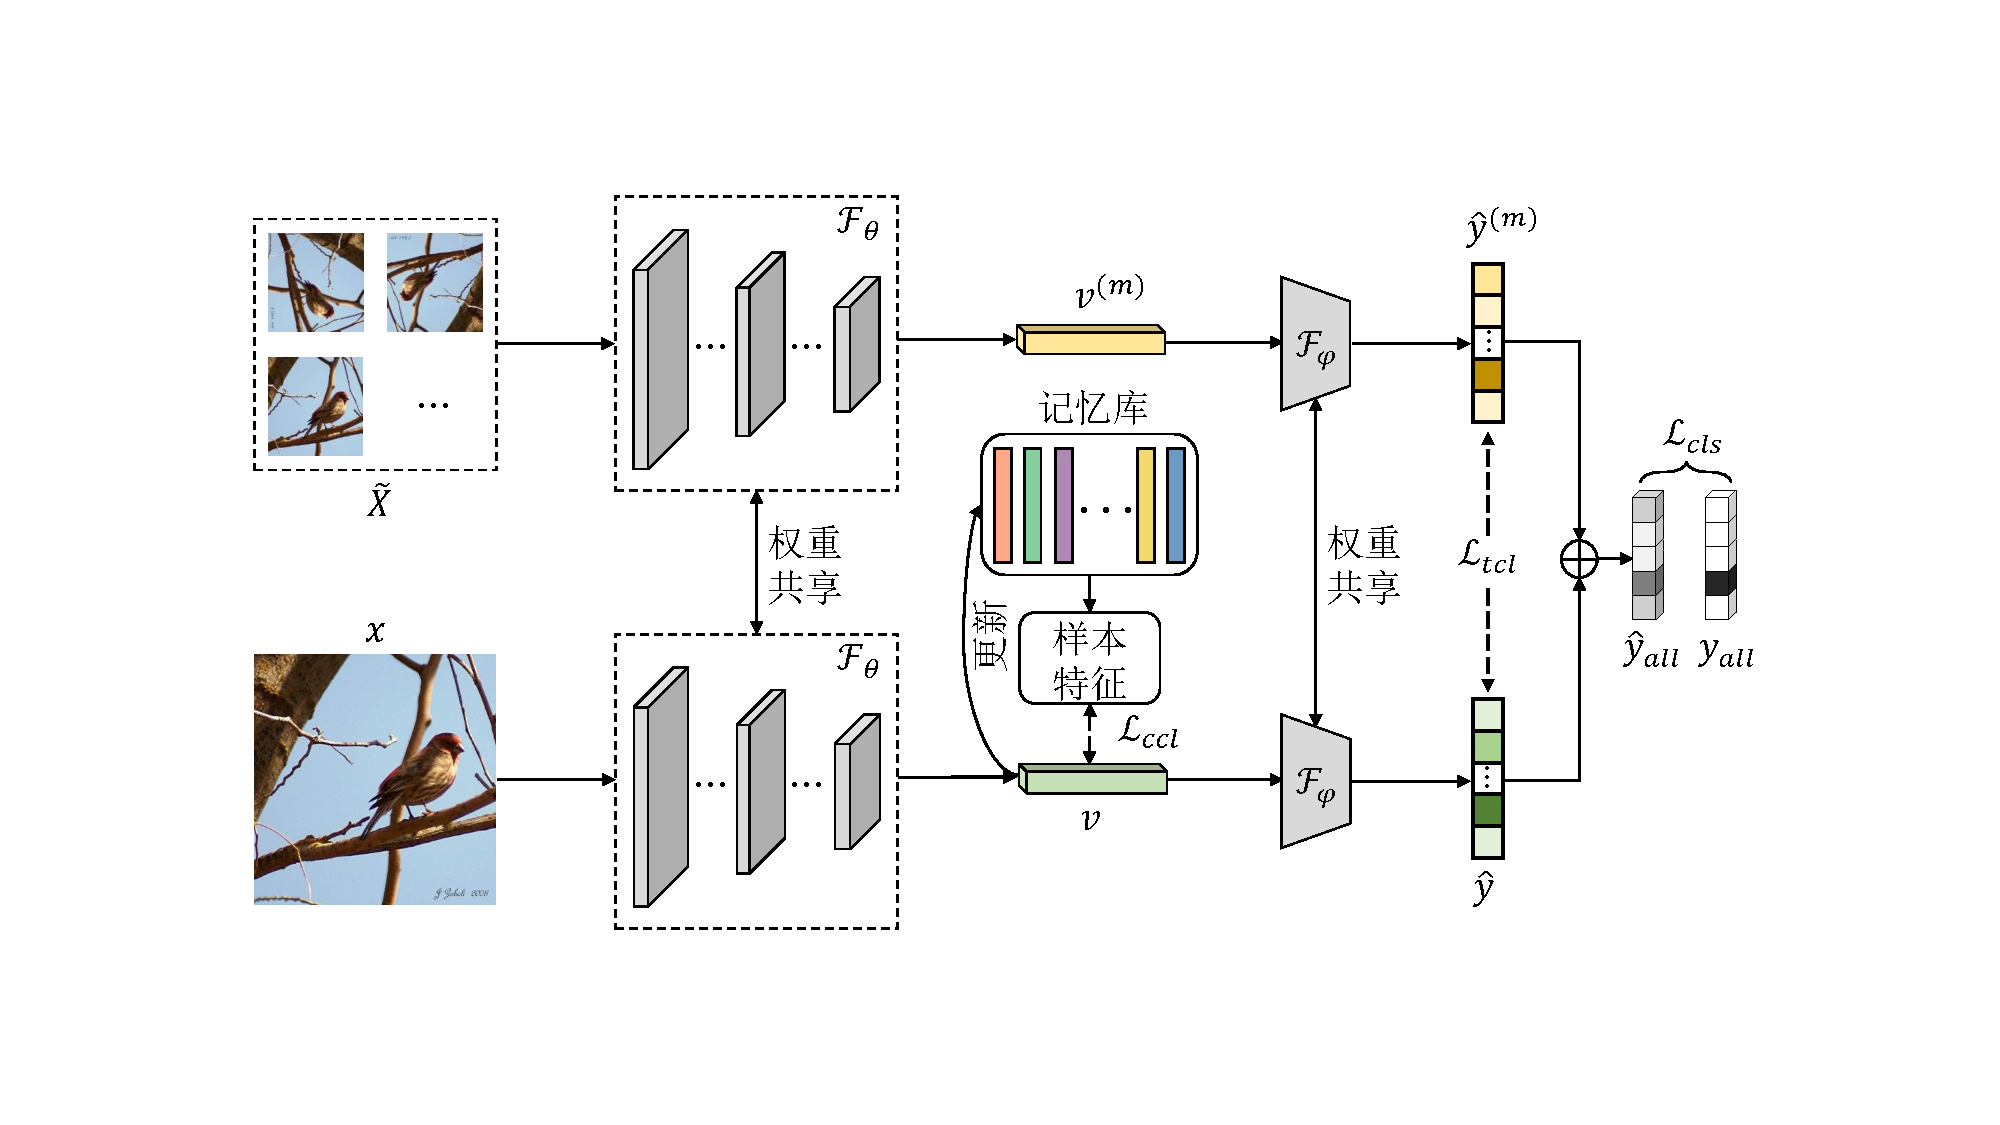
\includegraphics[width=1.0\columnwidth]{figures/MGSRCL/model.pdf}
% \captionsetup{justification=justified,singlelinecheck=false}
\bicaption[多粒度样本关系对比学习模型示意图]{多粒度样本关系对比学习模型(MGSRCL)示意图。它包含一个特征提取网络$\mathcal{F}_{\theta}$和一个分类器$\mathcal{F}_{\varphi}$。在此图中,$v$和$v^{(m)}$代表原始图像$x$及其第$m$个变换版本$x^{(m)}$的特征,其中$x^{(m)} \in \widehat{X}$。$\bigoplus$是一个连接操作,用于对原始图像的预测输出$\widehat{y}$与$M$个变换的预测输出${\widehat{y}^{(1)}, ..., \widehat{y}^{(m)}, ..., \widehat{y}^{(M)}}$进行连接。记忆库(Memory Bank)用于存储特征。$\mathcal{L}_{cls}$,$\mathcal{L}_{tcl}$和$\mathcal{L}_{ccl}$分别是分类损失、变换一致性学习(TCL)损失和类对比学习(CCL)损失。为了便于阅读,此图中没有展示自监督模块。}[Illustration of Multi-Grained Sample Relation Contrastive Learning (MGSRCL) model]{Illustration of Multi-Grained Sample Relation Contrastive Learning (MGSRCL) model. It contains a feature extraction network $\mathcal{F}_{\theta}$ and a classifier $\mathcal{F}_{\varphi}$. In this figure, $v$ and $v^{(m)}$ represent the features of the original image $x$ and its $m$-th transformed version $x^{(m)}$,where $x^{(m)} \in \widehat{X}$. $\bigoplus$ is a concatenation operator for the predicted output $\widehat{y}$ of the original image and the predicted outputs $\{\widehat{y}^{(1)}, ..., \widehat{y}^{(m)}, ..., \widehat{y}^{(M)}$\} of $M$ transformations. Memory bank is used to store the features. $\mathcal{L}_{cls}$, $\mathcal{L}_{tcl}$, and $\mathcal{L}_{ccl}$ are the classification loss, transformation consistency learning (TCL) loss, and class contrastive learning (CCL) loss, respectively. For the sake of legibility, the self-supervised module is not shown in this image.}
\label{figure3: model}
\end{figure}

\subsection[\hspace{-2pt}整体框架]{{\heiti\zihao{4} \hspace{-8pt}整体框架}}\label{section3: 整体框架}

本章重新审视了对比学习中的样本关系,并根据样本关系粒度的不同将其划分为三种类型:同一样本在不同变换下的样本内关系(intra-sample relation)、同类样本的类内关系(intra-class relation),以及不同类样本的类间关系(inter-class relation)。基于此,本章提出了一种新颖的多粒度样本关系对比学习方法(Multi-Grained Sample Relation Contrastive Learning,简称MGSRCL),通过对少样本分类中不同粒度的样本关系进行建模从而获得了一个强大的特征提取网络。如图\ref{figure3: model}所示,MGSRCL模型包含三个主要部分:基础特征学习网络(Base Feature Learning Network,简称Base)、变换一致性学习(Transformation Consistency Learning,简称TCL)模块和类对比学习(Class Contrastive Learning,简称CCL)模块。具体而言,基础特征学习网络是通过一般图像分类任务训练的神经网络。TCL模块旨在确保同一样本的不同变换版本具有一致的语义内容。而CCL则用于确保同类样本具有相似的语义内容,以及非同类样本具有不同的语义内容。接下来,本节将对MGSRCL方法的每个部分进行更为详细的阐述。

\subsection[\hspace{-2pt}基础特征学习网络]{{\heiti\zihao{4} \hspace{-8pt}基础特征学习网络}}\label{section3: 基础特征学习网络}

如图\ref{figure3: model}所示,特征提取网络,表示为带有参数$\theta$的$\mathcal{F}_{\theta}$,被用于提取图像特征。设$(x, y)\in \mathcal{D}_{base}$表示从$\mathcal{D}_{base}$中采样的图像及其对应的标签。图像$x$的特征向量$v$可以通过$\mathcal{F}_{\theta}$获得:$v=\mathcal{F}_{\theta}(x)$。然后,使用参数为$\varphi$的分类器$\mathcal{F}_{\varphi}$,将特征向量$v$投影到标签空间,以获得预测的置信度分数$p$:$p=\mathcal{F}_{\varphi}(v)$。最后,通过在$p$上应用Softmax函数,可以得到预测概率输出$\widehat{y}$:$\widehat{y}=\text{Softmax}(p)$。基础特征学习网络的参数$\theta$和$\varphi$通过最小化整个基类数据集$\mathcal{D}_{base}$上的分类损失$\mathcal{L}_{cls}$来进行优化,其可以表示为以下公式,
\begin{equation}
\label{equation3:3.2}
  \mathcal{L}_{cls} = - \frac{1}{|\mathcal{D}_{base}|}\sum_{\{x,y\}\in \mathcal{D}_{base}}y\log\widehat{y}.
\end{equation}

为了防止在训练集上过拟合,许多方法\cite{IER, PAL, SSLforFSL}引入了变换样本参与训练,并使用自监督学习技术预测在训练过程中对图像执行了哪种变换以增强网络的特征提取能力。遵循这些方法,本文也添加了一个由多层感知机(Multilayer Perceptron,简称MLP)构成的自监督(Self-Supervised,简称SS)模块。设$\widetilde{X}=\{\widetilde{x}^{(1)}, ..., \widetilde{x}^{(M)}\}$为一张图像的变换版本集合,其中$M$表示变换样本的总数,$\widetilde{x}^{(m)}$表示图像的第$m$个变换版本。$\widetilde{X}$可以通过在图像上应用一系列变换(如裁剪、调整大小、旋转等数据增强操作)获得。变换后的图像$\widetilde{X}$和原始图像$x$同时输入模型,用于分类和自监督任务。自监督任务的目标是识别图像进行了哪种变换,其损失$\mathcal{L}_{ss}$表示为以下公式,
\begin{equation}
\label{equation3:3.3}
  \mathcal{L}_{ss} = - \frac{1}{|\mathcal{D}_{base}|}\frac{1}{M+1}\sum_{x \in \mathcal{D}_{base}}\sum_{m=0}^{M}s^{(m)}\log\widehat{s}^{(m)},
\end{equation}
其中$\widehat{s}^{(m)}$和$s^{(m)}$分别表示自监督任务中第$m$个变换版本的预测概率输出和真实标签。$s^{(0)}$是原始图像$x$的自监督标签。此外,增加了变换样本之后的分类损失可以重新定义为以下公式,
\begin{equation}
\label{equation3:3.4}
  \mathcal{L}_{cls} = - \frac{1}{|\mathcal{D}_{base}|}\frac{1}{M+1}\sum_{x \in \mathcal{D}_{base}}\sum_{m=0}^{M}y^{(m)}\log\widehat{y}^{(m)},
\end{equation}
$\widehat{y}^{(m)}$表示分类任务中的预测概率输出,$y^{(m)}$表示分类任务的真实标签。

最后,基础特征学习网络的损失$\mathcal{L}_{base}$可以写为分类损失$\mathcal{L}_{cls}$和自监督损失$\mathcal{L}_{ss}$之和,
\begin{equation}
\label{equation3:3.5}
  \mathcal{L}_{base} = \mathcal{L}_{cls} + \mathcal{L}_{ss}.
\end{equation}

\subsection[\hspace{-2pt}多粒度样本关系对比学习算法]{{\heiti\zihao{4} \hspace{-8pt}多粒度样本关系对比学习算法}}\label{section3: 多粒度样本关系对比学习算法}

\textbf{(1)变换一致性学习}

一个样本图像与其变换版本包含完全相同的对象和背景,仅因为进行了数据增强而使得图像在旋转角度、明暗、颜色等方面发生变化,但其内在的类别属性和语义内容应保持不变。为了实现这一目标,本文设计了一个变换一致性学习(Transformation Consistency Learning,简称TCL)模块,以约束同一样本不同变换版本的样本内关系。TCL模块通过约束一个样本和其变换版本的预测输出相同来确保它们具有一致的语义内容。这是因为预测输出反映了样本在每个类别中的预测概率,这些概率不仅表示了模型对于样本属于各个类别的置信度,而且深入地揭示了样本的本质属性——语义内容。

本章方法将一个样本与其变换版本同时输入网络,并在预测标签输出层面计算它们的TCL损失。这里,本文使用Jensen-Shannon散度\cite{JS1, JS2}作为TCL损失,它能够衡量两个概率分布的差异,通过最小化两个预测标签的输出,可以使其概率分布一致,从而达到使样本和其变换版本具有一致语义内容的目的。TCL损失可以写为以下公式,
\begin{equation}
\label{equation3:3.6}
  \mathcal{L}_{tcl} = \frac{1}{|\mathcal{D}_{base}|}\sum_{x \in \mathcal{D}_{base}}\frac{1}{M}\sum_{m=1}^{M}JS(\widehat{y}_{\tau_1}, \widehat{y}_{\tau_1}^{(m)}),
\end{equation}
其中$\widehat{y}_{\tau_1}$和$\widehat{y}_{\tau_1}^{(m)}$分别是原始图像和第$m$个变换图像的平滑标签输出。它们通过以下公式获得,
\begin{equation}
\label{equation3:3.7}
  \widehat{y}_{\tau_1} = \text{Softmax}(p/\tau_1),
\end{equation}
此公式中$p = \mathcal{F}_{\varphi}(\mathcal{F}_{\theta}(x))$,$\tau_1$是一个温度参数,本文在实验中将其设置为$4.0$。使用平滑标签输出的原因在于不同变换的输出不仅需要在最大预测概率的类别上保持一致,而且需要在所有其他类别上也保持一致,以确保它们具有完全相同的语义内容,而平滑标签输出可以提供更多关于概率分布差异的信息。

\textbf{(2)类对比学习}

同类样本虽然图像内包含了同一个类别的物体,但物体及其背景与同一图像不同变换版本相比差异性较大,因此其预测概率输出之间差异也会较大。如果强行将其预测输出进行对齐,可能会使得网络为了学习此种强关系而导致模型崩塌。但在另一方面,同类样本间距离比不同类样本间距离更近是毋庸置疑的。因此,本文采用类对比学习(Class Contrastive Learning,简称CCL)以一种相对距离的形式约束同类样本的类内关系和不同类样本的类间关系。CCL模块通过最大化同类样本特征的相似性,同时最小化不同类样本特征的相似性来在特征空间拉近同类样本,推远不同类样本。

与之前对比学习不同,CCL模块为了将样本和其他每个不同类间的距离推远,对于每张图像都需要该图像的一个同类样本以及其他每个类别的不同类样本(之前对比学习通常随机采样,这使得每个批次计算损失时不同类样本可能仅来自部分不同类别)。为了实现这一目标并加快训练速度,本文使用了一个记忆库(Memory Bank)来存储和从中采样图像特征,记忆库存储了所有图像的特征。在一个批次中,CCL模块从记忆库中为每类图像随机采样一个样本的特征。CCL损失可以定义为,
\begin{equation}
\label{equation3:3.8}
  \mathcal{L}_{ccl} = \frac{1}{|\mathcal{D}_{base}|}\sum_{x \in \mathcal{D}_{base}}-\log \frac{\text{exp}(\frac{cos(v, v^\prime)}{\tau_2})}{\sum_{i=1}^{|\mathcal{C}_{base}|}{\text{exp}(\frac{cos(v, v_i)}{\tau_2})}},
\end{equation}
其中$|\mathcal{C}_{base}|$和$|\mathcal{D}_{base}|$表示基类的类别数量和样本数量,$v$和$v^\prime$分别是某个样本及其同类样本的特征,$v_i$代表来自第$i$类的样本的特征。这里$v^\prime$和$v_i$是从记忆库中采样的。$cos(\cdot)$是余弦相似度,$\text{exp}(\cdot)$为以e为底的指数函数。而$\tau_2$是一个温度参数,本文按照\cite{SimCLR, SupCon}的实验设置将其设为$0.1$。此外,记忆库的更新方式为,
\begin{equation}
\label{equation3:3.9}
  v_{k} = r\times v_k + (1 - r)\times v_q,
\end{equation}
$v_q$和$v_k$分别代表在当前小批次中获得的图像特征以及在记忆库中存储的相同图像的特征,$r$用于调整记忆库的更新速度,按照IER方法\cite{IER}的实验,本文将其设置为$0.99$。在训练阶段,记忆库每一轮训练过程都会完全更新一遍。

\subsection[\hspace{-2pt}模型优化]{{\heiti\zihao{4} \hspace{-8pt}模型优化}}\label{section3: 模型优化}
结合公式\ref{equation3:3.5}、\ref{equation3:3.6}和\ref{equation3:3.8},本章提出的MGSRCL模型总体损失函数可以表示为以下公式,
\begin{equation}
\label{equation3:3.10}
  \mathcal{L}_{total} = \mathcal{L}_{base} + \alpha \cdot \mathcal{L}_{tcl} + \beta \cdot \mathcal{L}_{ccl},
\end{equation}
其中$\alpha$和$\beta$是用于平衡不同损失的超参数,分别表示TCL模块和CCL模块的损失权重。

MGSRCL模型通过在整个基类数据集上最小化上述损失函数对模型参数进行联合优化。通过建模多个粒度的样本关系,可以有效地增强模型的特征提取能力和泛化能力,帮助模型捕获更具判别性的特征,从而提高模型在新类$\mathcal{D}_{novel}$上的分类性能。

\subsection[\hspace{-2pt}模型推理]{{\heiti\zihao{4} \hspace{-8pt}模型推理}}\label{section3: 模型推理}
模型在基类数据集$\mathcal{D}_{base}$训练完成之后,在测试阶段,将会冻结MGSRCL模型特征提取网络的所有参数,并通过解决来自新类$\mathcal{D}_{novel}$的大量少样本分类任务来评估模型性能。在每个任务$\mathcal{T}$的推理过程中,本文使用特征提取网络$\mathcal{F}_{\theta}$来获得支持集$\mathcal{S}_\mathcal{T}$和查询集$\mathcal{Q}_\mathcal{T}$的图像特征。然后,本文使用$\mathcal{S}_\mathcal{T}$的样本特征训练一个逻辑回归分类器$LC$,并对$\mathcal{Q}_\mathcal{T}$中的样本进行分类,最后将在多个少样本分类任务上的准确率平均值作为模型的评价指标。MGSRCL模型的推理过程如图\ref{figure3: 推理过程}所示。

\begin{figure}[h]
\centering
\captionsetup{font={small, stretch=1.312}}
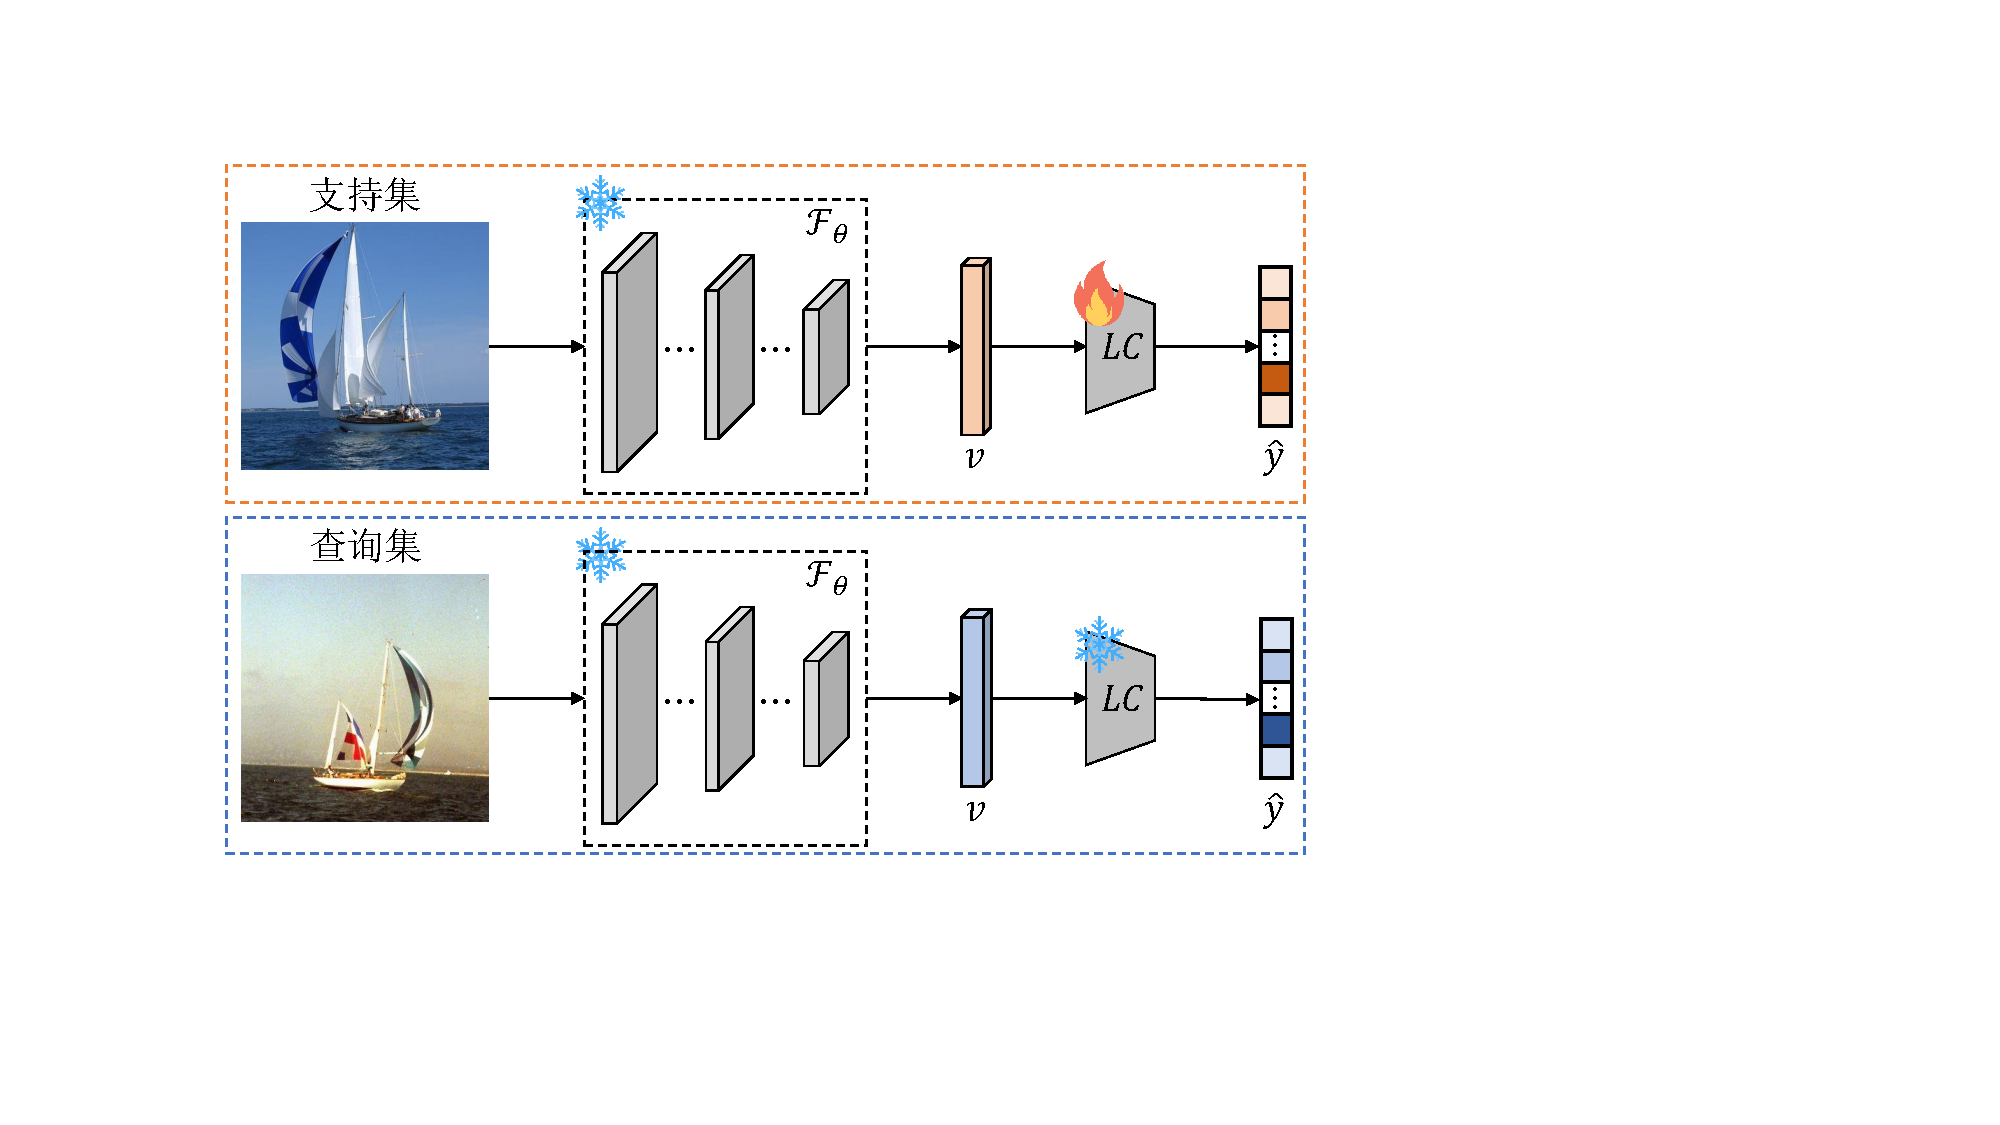
\includegraphics[width=0.8\columnwidth]{figures/MGSRCL/推理过程.pdf}
% \captionsetup{justification=justified,singlelinecheck=false}
\bicaption[MGSRCL模型推理过程示意图]{MGSRCL模型推理过程示意图。推理过程中,使用冻结参数的特征提取网络$\mathcal{F}_{\theta}$提取支持集与查询集的图像特征。其中,支持集特征被用来训练一个逻辑回归分类器$LC$,查询集特征则是用来测试分类器性能。}[Illustration of MGSRCL model inference process]{Illustration of MGSRCL model inference process. During the inference process, the feature extraction network $\mathcal{F}_{\theta}$ with frozen parameters is used to extract image features from both support set and query set. Herein, the support set features are utilized to train a logistic regression classifier $LC$, while the query set features are used to assess the classifier's performance.}
\vspace{-10pt}
\label{figure3: 推理过程}
\end{figure}

\section[\hspace{-2pt}实验设置及结果分析]{{\heiti\zihao{-3} \hspace{-8pt}实验设置及结果分析}}\label{section3: 实验设置及结果分析}
在本节中
\section[\hspace{-2pt}本章小结]{{\heiti\zihao{-3} \hspace{-8pt}本章小结}}\label{section3: 本章小结}

本章
